\documentclass{article}
\usepackage[a4paper,twoside,left=3cm,right=2cm,top=2cm,bottom=2cm]{geometry}
\usepackage[utf8]{inputenc}
\usepackage[french]{babel}
\usepackage{graphicx}
\usepackage{capt-of}
 
\usepackage{minted}

\title{Dossier technique\\Coopération de robots}
\author{Thibault Vernay, Victor Cazaux, Daphné Porteries}

\makeindex

\begin{document}

\maketitle

\tableofcontents

\section{Spécifications}

\subsection{Spécifications matérielles}

\subsection{Spécifications logicielles}

\section{Étude du matériel}

\subsection{Étude des capteurs et des actionneurs}

\subsubsection{Magnétomètre 3 axes}

Le magnétomètre que nous aurions aimé avoir est le MAG3110FCR1 qui est un composant nécessitant la création d'une carte d'acceuil avec des condensateurs de découplages pour les alimentations (dont les valeurs sont spécifiées dans la documentation du composant). Ce composant utilise le protocole $I^2C$ qui permet d'utiliser que deux lignes, la ligne SDA et la ligne SCL réciproquement pour les données et pour l'horloge. Le composant en $I^2C$ dispose d'une adresse sur 7 bits aligné à gauche à laquelle il faut ajouté le bit d'écriture ou de lecture pour en faire une information sur 8 bits. En plus de l'alimentation et des lignes destinées à l'$I^2C$ ce capteur possède une ligne destinée aux interruptions.

\begin{center}
  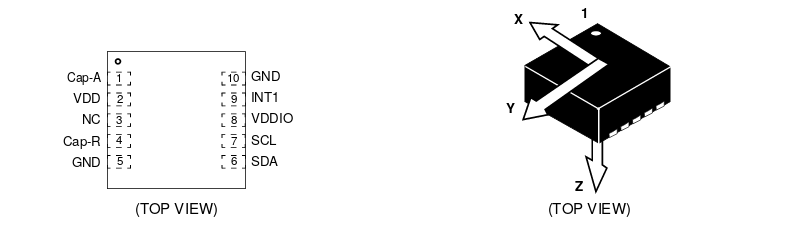
\includegraphics[width=17cm]{mag_schematic.png}
  \captionof{figure}{Schématique du composant}
\end{center}

Ce capteur utilise l'effet Hall, mais nous n'avons pas vraiment eu le temps d'en parfaire l'étude.

\subsection{Moteurs à courant continus et pont en H}

\subsection{Capteur de proximité infrarouge}

\subsection{Carte électronique}

\section{Étude du logiciel}

\subsection{Couche bas niveau}

\subsubsection{Configuration de STM32CubeMx}

Lors de l'utilisation d'une carte microcontrôleur telle que la STM8S ou la Nucléo STM32F3xx, il est nécessaire de configurer les ports, les pins, les différents registres des timers et des ADC avant même de commencer le code à proprement parlé. Dans le cas d'une carte STM32, il existe un outils très pratique nommé STM32CubeMX permettant de configurer préalablement les bons registres, ports et pins et de générer un ensemble de fichiers projet avec un Makefile adapté au projet. \\

Les fichiers s'organisent de la manière suivante~: \\
\begin{itemize}
  \item fichier ``main'' contenant l'initialisation de la carte~;
  \item fichiers contenant les fonctions de la ``HAL'' pour chaque module de la carte. \\
\end{itemize}

À chaque génération de projet, STM32CubeMx va inclure les bonnes bibliothèques au main et au Makefile. Par exemple si j'allume l'UART2 avec la configuration STM32CubeMX, le fichier stm32f3xx\_hal\_uart.h sera inclus et son .c associé sera compilé. La ``HAL'' (Hardware Abstraction Layout) est comme son nom l'indique une couche d'abstraction matérielle qui va se charger de mettre les bonnes valeurs dans les bons registres lors de l'initialisation mais également lors de l'utilisation. Elle embarque donc un certain nombre de fonctions générique de manipulation du matériel facilitant l'utilisation de la carte. La mise en place de la HAL s'illustre de la manière suivante~:\\

\begin{center}
  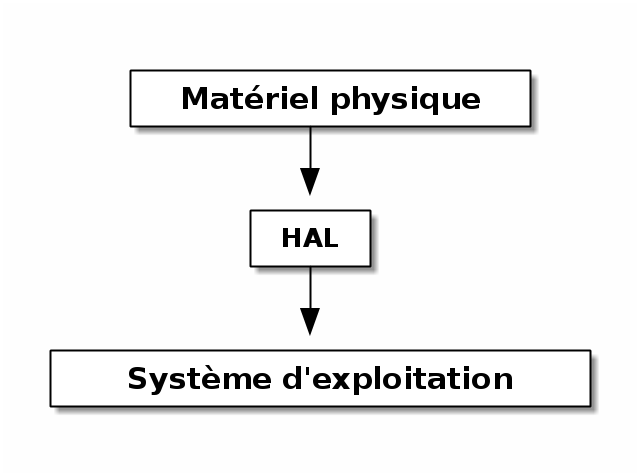
\includegraphics[height=5cm]{diag_HAL.png}
\end{center}

STM32CubeMx va aussi permettre autre chose~: la mise en place d'un OS temps réel nommé FreeRTOS permettant de paralléliser les tâches. Ainsi nous allons créer plusieurs tâches avec cet OS et profiter de sa gestion simplifiée des temporisations. Il faudra également gérer le HEAP et la taille de STACK lors de la mise en place de celui-ci. La ``STACK'' est la taille dans la mémoire maximum que peu prendre le programme lors de son exécution tandis que le HEAP existe lors de cas d'allocations dynamiques de la mémoire. Dans le cas de FreeRTOS toutes tâche créée est allouée dynamiquement dans la mémoire en fonction de la taille de sa stack notamment. Il faut donc penser à avoir de la marge côté heap et tester quelles valeurs maximale la carte accepte en fonction de la taille de sa RAM. La valeur max n'est pas mentionnée dans la doc, il faut donc tester empiriquement car une valeur trop élevée du Heap pose des problèmes lors du linkage et crée une erreur de ``RAM overflowed''. \\

Niveau mmatériel, trois tâches indépendantes serons créées~: une pour l'ADC, une pour les moteurs et une pour la gestion de l'UART. Nous parlerons dans cette partie des deux premières.

\subsubsection{Commande des actionneurs}

Les moteurs courant continus sont commandés à l'aide d'un pont en H nécessitant de deux pins de commandes par moteur et d'un PWM par moteur. Le principe du PWM est assez simple, il est rattaché au principe de rapport cyclique. On va donc utiliser un timer qui au lieu de compter simplement jusqu'à la valeur du registre ARR, va avoir une deuxième valeur de comparaison inférieure à celle de l'ARR. Le signal du PWM change de polarité quand le timer atteint cette valeur et quand le timer fini de compter, ainsi on a un signal carré avec un rapport cyclique variable en fonction de cette valeur de comparaison. \\

Nous avons donc plusieurs calculs à notre disposition pour avoir une certaine fréquence de PWM et un certain rapport cyclique~: \\

\begin{center}
  $timer\_tick\_frequency = Timer\_default\_set \div ( prescaller\_set + 1 )$ \\
  $PWM\_frequency = timer\_tick\_frequency \div ( TIM\_period + 1 ) $ \\
  $TIM\_period = timer\_tick\_frequency \div PWM\_frequency - 1 $ \\
  $pulse\_lenght = ((TIM\_period + 1) \times DutyCycle) \div 100 - 1$ \\
\end{center} 

où ``DutyCycle'' est une valeur exprimée en pourcent qui représente notre rapport cyclique. Ainsi avec notre horloge à 64MHz nous choisissons un prescaller de $999$ (pour diviser la fréquence du timer par $1000$, on veut maintenant une fréquence de PWM de 100Hz, on effectue donc la troisième ligne de calcul et on trouve que la valeur de l'ARR doit être de $639$ pour atteindre cette fréquence. Maintenant si on veut un rapport cyclique de $0,25$ il faut un ``DutyCycle'' de $25\%$ on obtient donc que $159$ est la valeur à mettre pour la comparaison du PWM. Si nous voulons que nos deux moteurs aillent à la même vitesse il faut donc que les deux PWM soient configurés à l'identique. Nous utiliserons ici qu'un seul timer, le timer 2 qui possède quatre lignes sur lesquelles on peut configurer des PWM, ici la ligne 1 et 4. \\

D'après la datasheet, pour que le moteur fonctionne et s'allume, il faut que la ligne reliée à l'entrée standby soit à l'état haut et que les deux lignes d'entrées soient de valeur opposées. Ainsi on initialise la ligne reliée à l'entrée standby à l'état haut et on crée diverse fonctions permettant d'allumer les moteurs dans un sens ou dans l'autre en fonction du tableau d'états fourni dans la datasheet du pont en H. Ces fonctions vont permettre de créer les autres fonctions de déplacements~: avancer, reculer, touner à droite ou à gauche. Moduler le pwm grâce aux fonctions de la HAL permet également de faire des routines d'accélération et de décélération.

\subsubsection{Configuration des capteurs}

Le capteur de détection des distances est un capteur infrarouge SHARP. À partir de sa véritable distance minimale pour laquelle la tension renvoyée est maximale il effectue une courbe de tension à allure exponentielle inverse. La valeur en tension doit être récupérée par une entrée analogique, puis traduite en fonction de la précision voulue (ici sur 12 bits donc en valeur numérique entre $0$ et $4095$ pour $3,3V$) et ensuite étalonné pour que la valeur récupérée par la carte soit traduite en distance. Pour travailler plutôt avec des variables dites ``drapeau'' nous utiliserons ici l'ADC avec des interruptions toutes les 10 millisecondes (après une tentative ratée d'utilisation de la DMA avec un timer pour commander l'ADC, l'erreur est encore inconnue).\\

Pour ce faire il faut configurer l'ADC avec une résolution de 12 bits. augmenter le nombre de cycles quand le temps entre deux conversions devient faible (ici le temps entre deux conversions sera de 10 millisecondes) et activer les interruptions avec NVIC qui est un module de la carte gérant les interruptions. Utiliser la conversion continue ne marchait pas dans notre cas sans véritables explications, nous avons décidé de nous en passer. Niveau code, il faut démarrer l'ADC avec la HAL et les interruptions, récupérer dans le code le prototype de la fonction ``HAL\_ADC\_ConvCompltCallback'' qui s'executera à chaque fois qu'une conversion sera terminée. Cette fonction est déclarée en ``\_\_weak'' ce qui signifie que si elle est déclarée dans un autre fichier, lors de la compilation seule celle qui n'a pas le mot clé ``\_\_weak'' sera compilée, l'autre sera ignorée. Elle est vide, il faut donc coder son contenu. Ici nous décidons d'utiliser des variables drapeau pour indiquer l'état de la variable qui stocke la donnée. Cette fonction positionne donc l'état du drapeau à 1 et récupère la valeur de l'ADC dans une variable globale au fichier. \\

La tâche associée à l'ADC n'a plus qu'à vérifier l'état du drapeau, traiter la valeur de l'ADC et remettre la valeur du drapeau à 0.

\subsubsection{Fonctions primitives}

Les fonctions primitives sont les fonctions proches du matériel qui sont données aux couches supérieures. Ici ces fonctions primitives sont au nombre de 5~: \\

\begin{itemize}
  \item avancer~;
  \item reculer~;
  \item pivoter à droite~;
  \item pivoter à gauche~;
  \item distance frontale. \\
\end{itemize}

Les fonctions de déplacement mettent en place l'allumage séparé des moteurs, la gestions du PWM avec les routines d'accélération et de décélération et les temporisations permettant pour les déplacement linéaires de parcourir 15 cm (longueur d'une case pour l'IA) et pour les fonctions tournante d'atteindre approximativement un angle de 90 degrés (difficile sans boussole). La fonction distance frontale quant à elle va prendre en compte non seulement la distance traduite du capteur, mais aussi la distance entre l'avant du robot et le placement de celui-ci mais risque des erreurs quand cette distance est inférieure à 5 cm (chute de tension brutale). 

\section{Couche communication}

\section{Couche intelligence artificielle}

\end{document}
